\chapter{Benutzerdokumentation}

\section{Installation}
Die Software wird als SEPGruppe11.zip ausgeliefert. Der erste Schritt ist die zip-Datei zu entpacken. Abhängig davon wo die zip-Datei entpackt wird, ist sicherzustellen, dass man sich im Ordner befindet,der den Ordner \emph{Quellcode} und die vier \emph{sh}-Dateien enthält.
Die Voraussetzung, dass die Software installiert werden kann, ist ein QT5 fähiger Compiler.
Um die Doxygen-Dokumentation erstellen zu können, muss Doxygen installiert sein.

\subsection{Linux}
\subsubsection{Installation}
Zur Installation unter Linux muss das Skript \emph{install.sh} ausgeführt werden. Gegebenenfalls muss das Skript mit den entsprechenden Rechten versehen werden, dies geschieht über den Befehl \emph{chmod 755 install.sh}. Danach kann man dann das fertige Programm mit dem Befehl \emph{make run} ausgeführt werden.
\subsubsection{Deinstallation}
Zur Deinstallation unter Linux muss das Skript \emph{deinstall.sh} ausgeführt werden. Gegebenenfalls muss das Skript mit den entsprechenden Rechten versehen werden, dies geschieht über den Befehl \emph{chmod 755 deinstall.sh}.

\subsection{Windows}
Zur Installation unter Windows muss die \emph{SEP\_WLeitung.pro} Datei im Ordner Code über Qt-creator geöffnet werden und dort compiliert werden.

\subsection{Doxygen} \label{Installation Doxygen}
\subsubsection{Linux}
Zur Estellung der Doxygen Dokumentation muss das Skript \emph{makeDoxygen.sh} ausgeführt werden. Anschließend muss die \emph{starteDoxygen}-Datei ausgeführt werden, um die Doxygen Dokumentation zu starten. Zur Bereinigung der Doxygen Dokumentation muss das Skript \emph{cleanDoxygen.sh} ausgeführt werden. Gegebenenfalls müssen die beiden Skripte mit den entsprechenden Rechten versehen werden, dies geschieht über die Befehle \emph{chmod 755 makedoxygen.sh} oder \emph{chmod 755 cleanDoxygen.sh}. 

\subsubsection{Windows}
Zur Erstellung muss im Doxy-Wizard die Konfigurationsdatei \emph{doxygen-config} geladen werden und dann der \emph{run}-Button betätigt werden.

\newpage
\section{Beispielsitzung}

Bevor der Benutzer eine Simulation startet, kann er die folgenden Einstellungen festlegen, um ein Simulationsexperiment zu spezifizieren:
\begin{itemize}
\item Temperaturleitkoeffizienten
\item Wärmequellen
\item Anfangs- und Randwerte
\item Diskretisierungsparameter
\end{itemize}
\noindent
Nach Start des Programms wird die graphische Benutzeroberfläche angezeigt.
\begin{figure}[H]
\centering
%\hspace{-1.75cm}
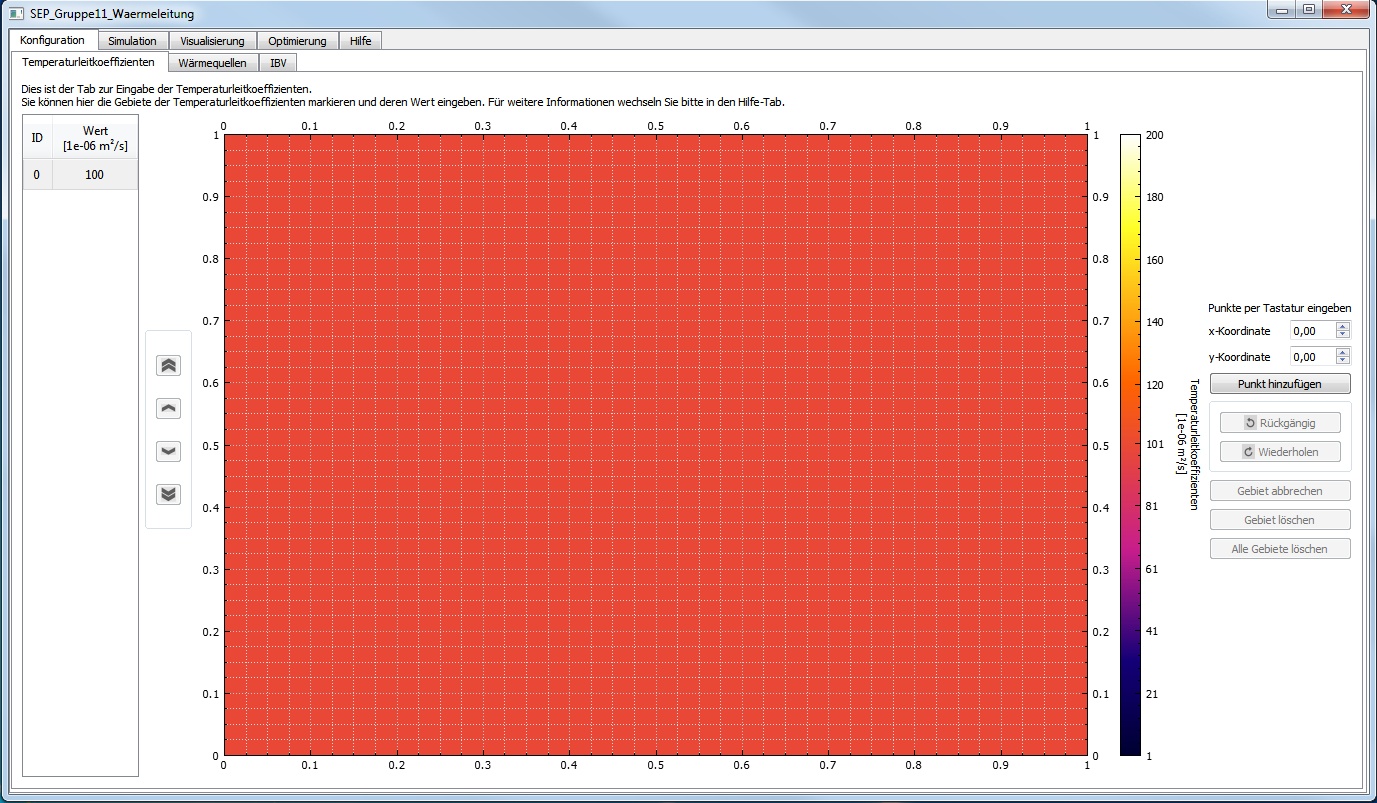
\includegraphics[scale=.5]{Bilder/StartAnzeige.png}\\
\caption{graphische Benutzeroberfläche}
\label{graphische Benutzeroberfläche}
\end{figure}

\newpage
\noindent
Im Temperaturleitkoeffizienten- und Wärmequellen-Tab kann der Benutzer Gebiete festlegen. In den beiden Tabs stehen dem Benutzer die folgenden Funktionalitäten zur Verfügung:\\


\noindent
Neues Gebiet hinzufügen:
Klicken Sie entweder mit der linken Maustaste an die gewünschte Stelle auf der Platte oder geben Sie die Koordinaten über die Felder 'x-Koordinate' und 'y-Koordinate' ein und bestätigen Sie mit 'Punkt hinzufügen'. Um die Eingabe eines Gebietes abzuschließen müssen Sie auf den Startpunkt des Gebietes klicken. Ein Gebiet ist nur dann korrekt, wenn es einfach wegzusammenhängend ist, d.h. Kanten dürfen sich nicht schneiden und es muss abgeschlossen sein. Wurde ein Gebiet korrekt eingegeben können Sie den Temperaturleitkoeffizienten (in $1e-06 m^2/s$) bzw den Wert der Wärmequelle zu diesem Gebiet eingeben.
\begin{figure}[H]
\centering
%\hspace{-1.75cm}
\includegraphics[scale=.25]{Bilder/GebietHinzufuegen.png}\\
\caption{Gebiet hinzufügen}
\label{Ein neues Gebiet hinzufügen}
\end{figure}

\newpage
\noindent
Einen Punkt rückgängig machen:
Um während der Eingabe eines neuen Gebietes einen Punkt rückgängig zu machen, klicken Sie auf den Knopf 'Rückgängig'.
\begin{figure}[H]
\centering
%\hspace{-1.75cm}
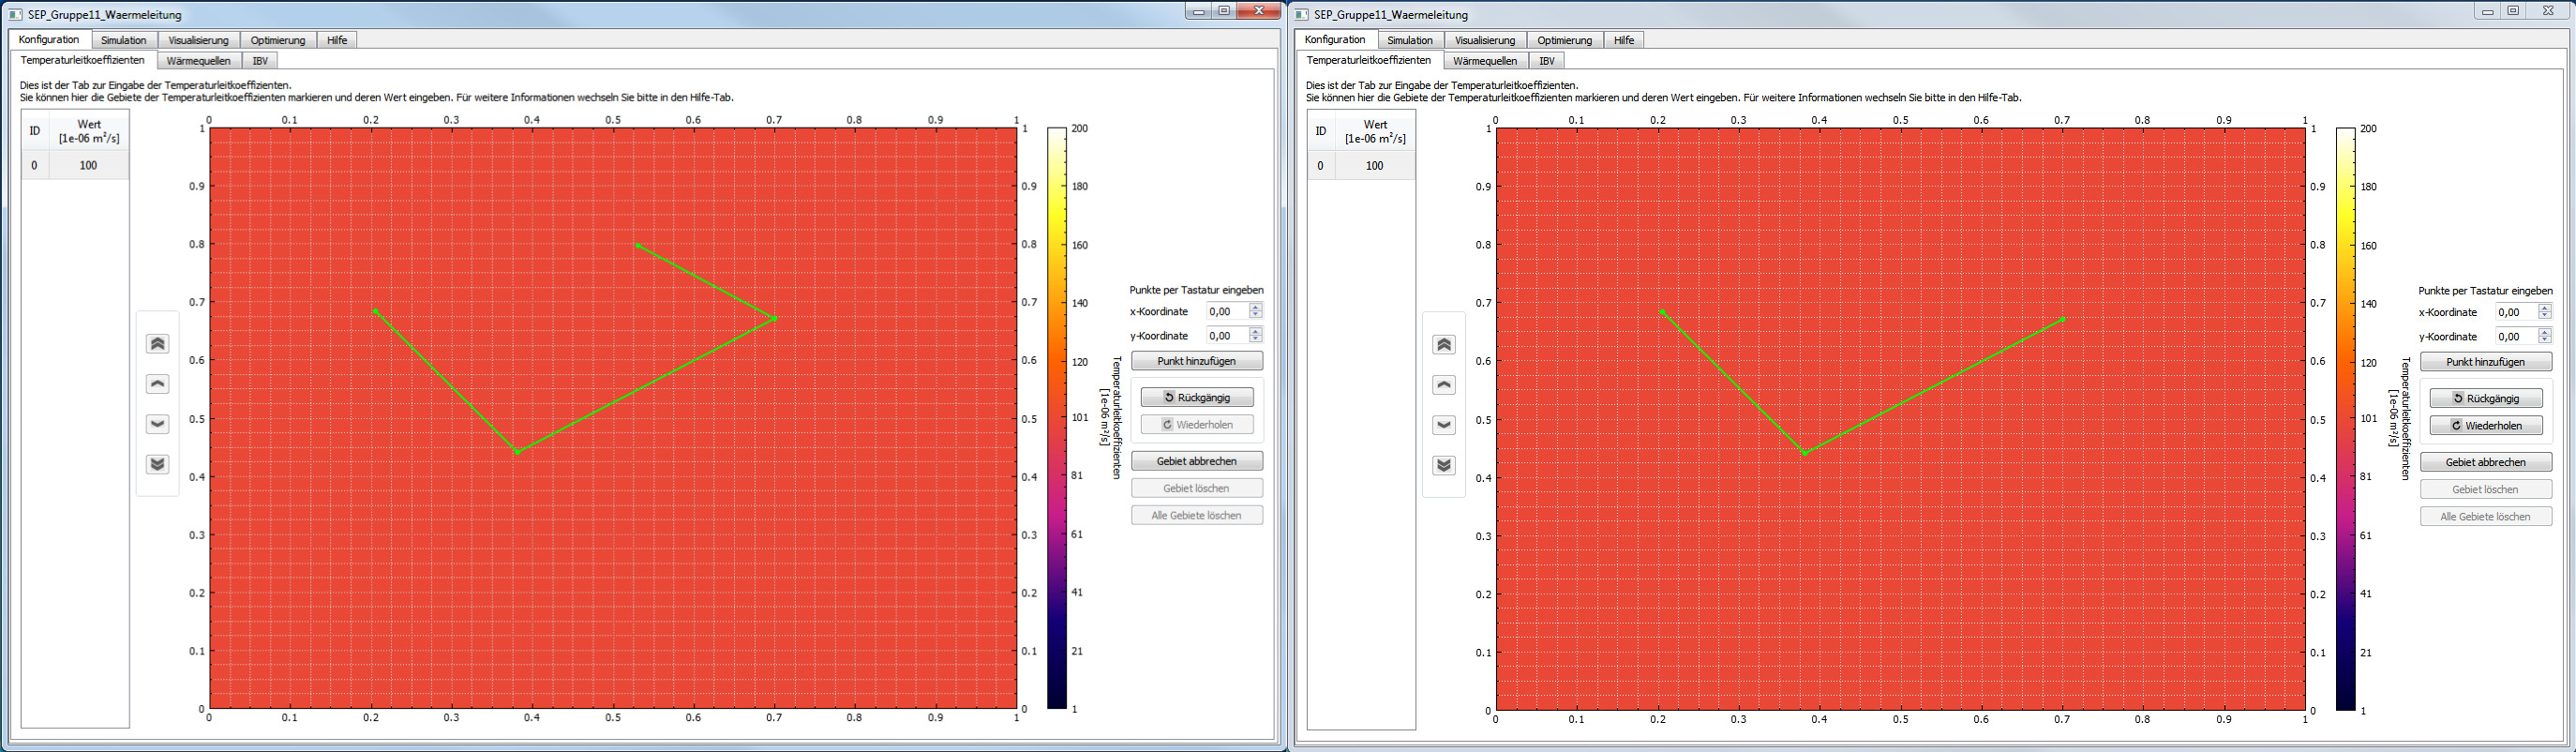
\includegraphics[scale=.25]{Bilder/PunktRueckgaengig.png}\\
\caption{Einen Punkt rückgängig machen}
\label{PunktRueckgaengig}
\end{figure}

\noindent
Ein Gebiet abbrechen: Um das aktuell begonnene Gebiet zu löschen, klcken Sie auf den Knopf 'Gebiet abbrechen'.
\begin{figure}[H]
\centering
%\hspace{-1.75cm}
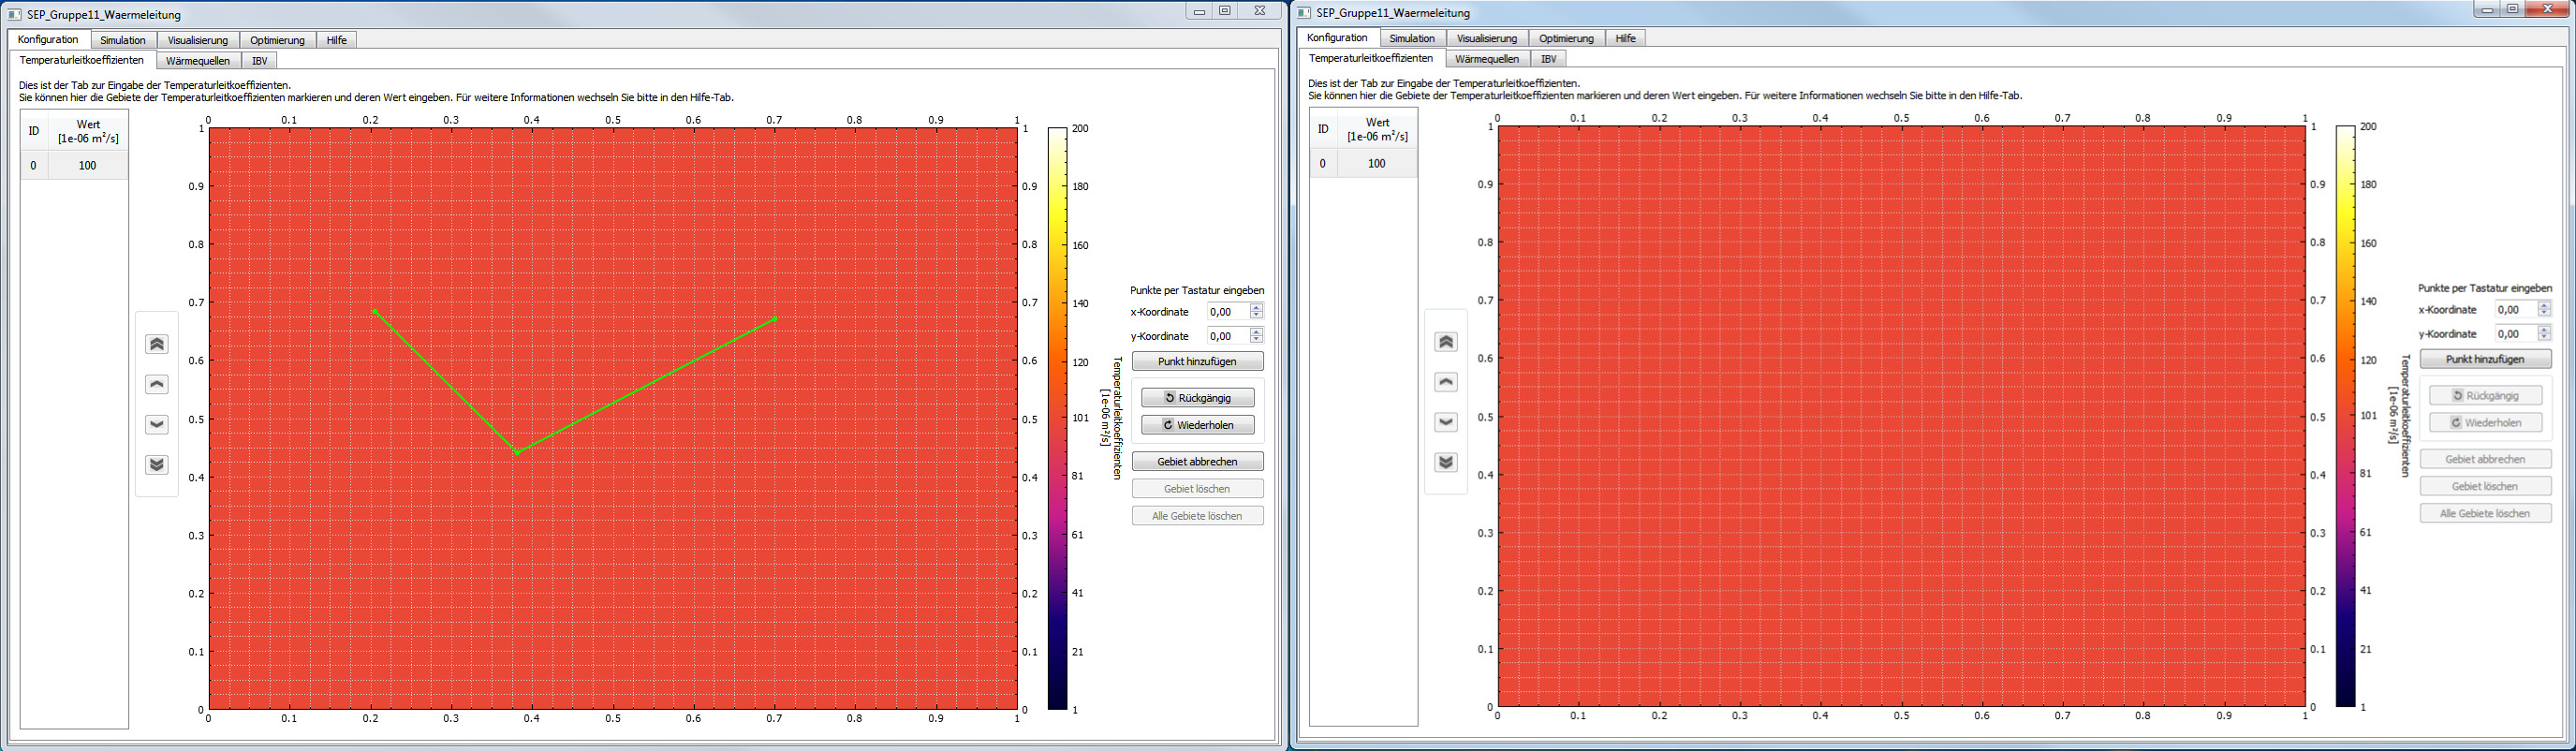
\includegraphics[scale=.25]{Bilder/GebietAbbrechen.png}\\
\caption{Ein Gebiet abbrechen}
\label{GebietAbbrechen}
\end{figure}

\noindent
Ein Gebiet löschen: Um ein beliebiges Gebiet zu löschen muss der Radio-Button 'Gebiet auswählen', aktiviert sein. Wählen Sie nun auf der Platte das Gebiet aus, welches Sie löschen wollen und klicken Sie anschließend auf den Knopf 'Gebiet löschen'.
\begin{figure}[H]
\centering
%\hspace{-1.75cm}
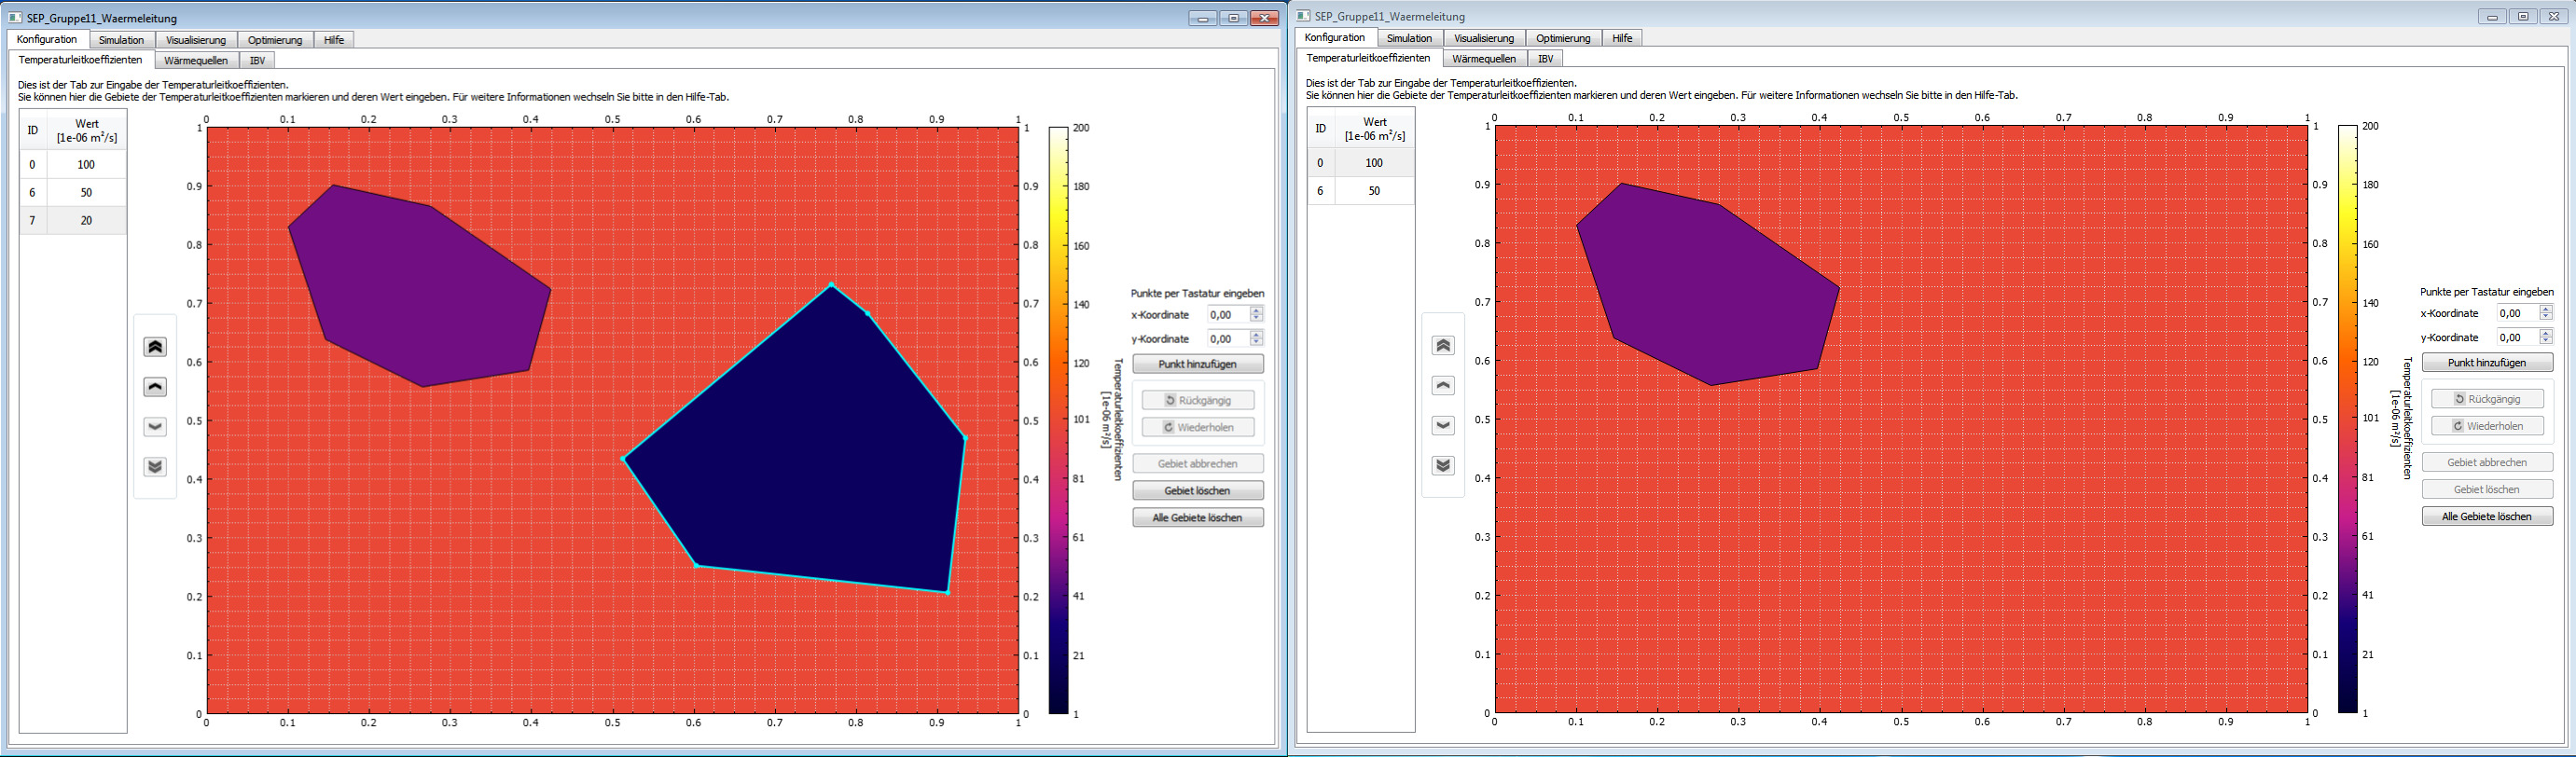
\includegraphics[scale=.25]{Bilder/GebietLoeschen.png}\\
\caption{Ein Gebiet löschen}
\label{GebietLoeschen}
\end{figure}

\newpage
\noindent
Alle Gebiete löschen: Um alle Gebiete zu löschen, klicken Sie auf den Knopf 'Alle Gebiete löschen'.
\begin{figure}[H]
\centering
%\hspace{-1.75cm}
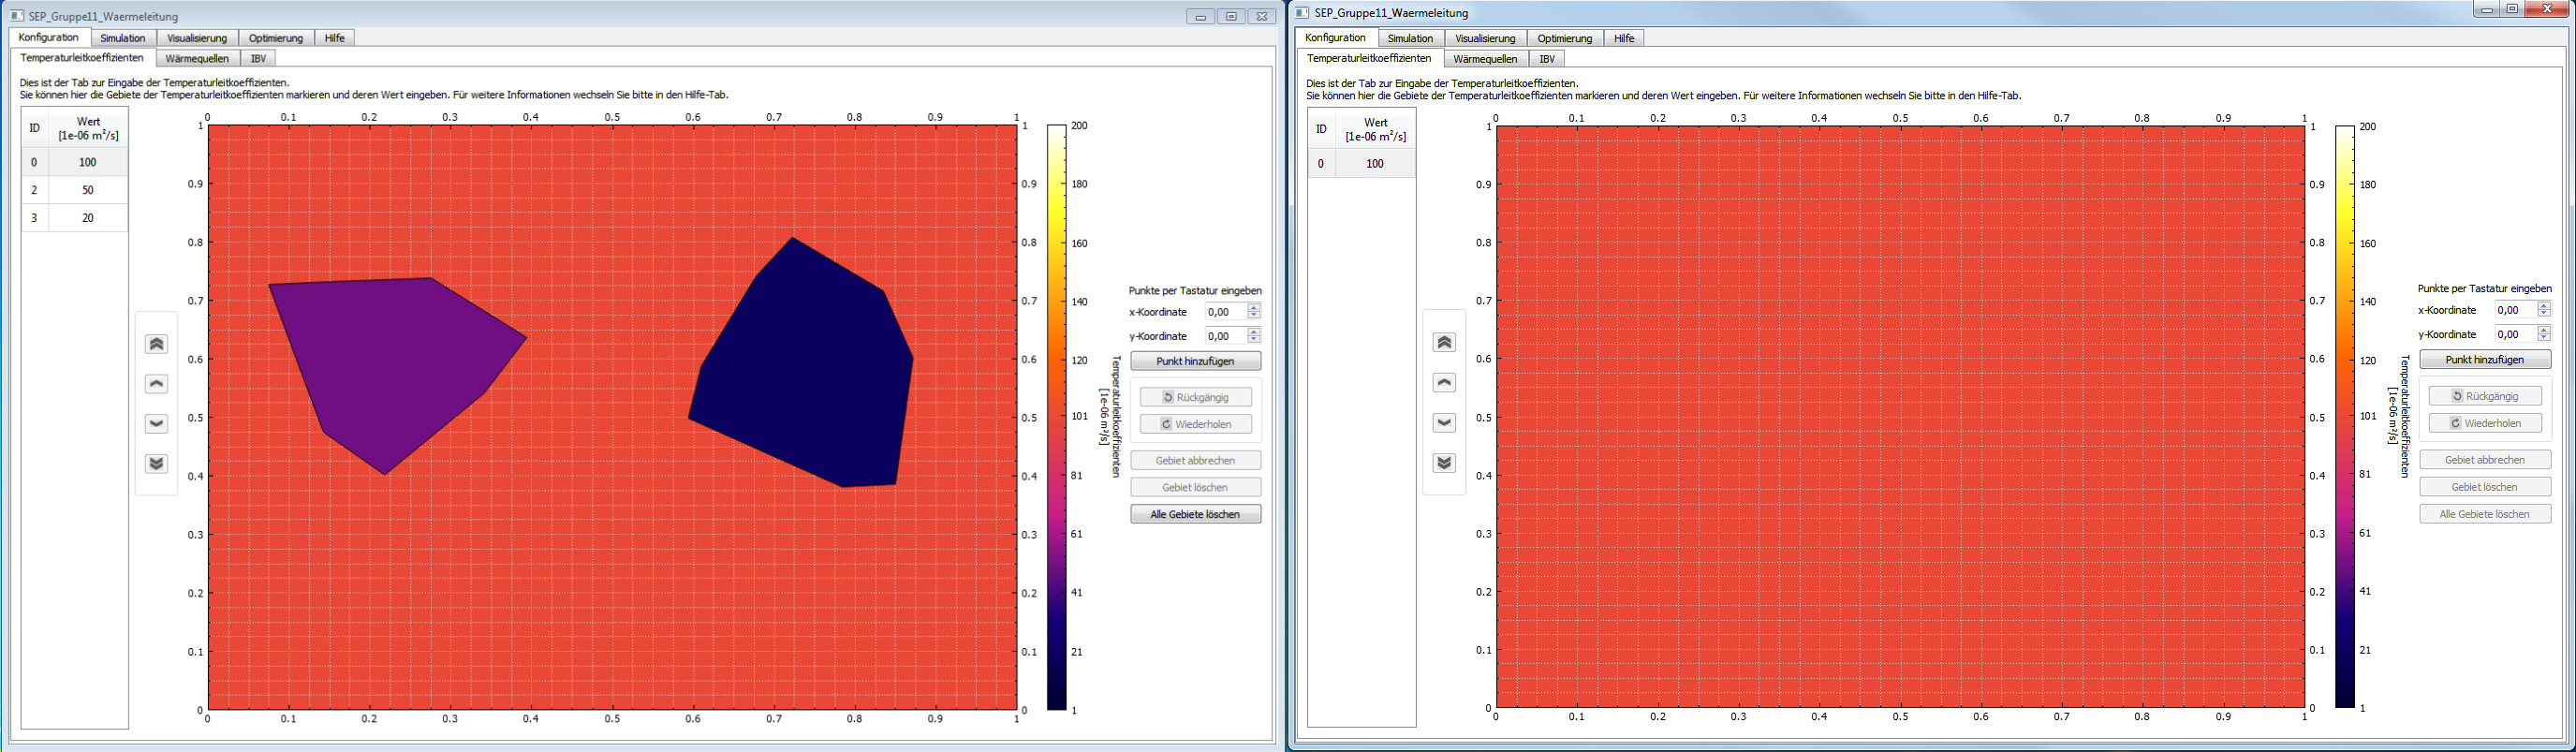
\includegraphics[scale=.25]{Bilder/AlleGebieteLoeschen.png}\\
\caption{Alle Gebiete löschen}
\label{AlleGebieteLoeschen}
\end{figure}

\noindent
Reihenfolge der Gebiet tauschen: Sie können die Reihenfolge der eingegebenen Gebiete in der Tabelle ändern. Hierfür muss mehr als ein Gebiet auf der Platte eingegeben worden sein. Klicken Sie entweder mit der rechten Maustaste auf das gewünschte Gebiet auf der Platte oder klicken Sie auf die Zeile des entsprechenden Gebietes um dieses zur markieren. Anschließend können Sie die Reihenfolge mit den Pfeiltasten neben der Tabelle ändern. Mit einem Klick auf den einfachen Pfeil wird das ausgewählte Gebiet entweder um eine Position nach oben oder nach unten in der Tabelle verschoben. Mit einem Klick auf den doppelten Pfeil wird das ausgewählte Gebiet entweder an den Anfang oder ans Ende der Tablle verschoben. Das Gebiet welches in der Tablle an letzter Position steht, wird auf der Platte als oberstes Gebiet angezeigt.
\begin{figure}[H]
\centering
%\hspace{-1.75cm}
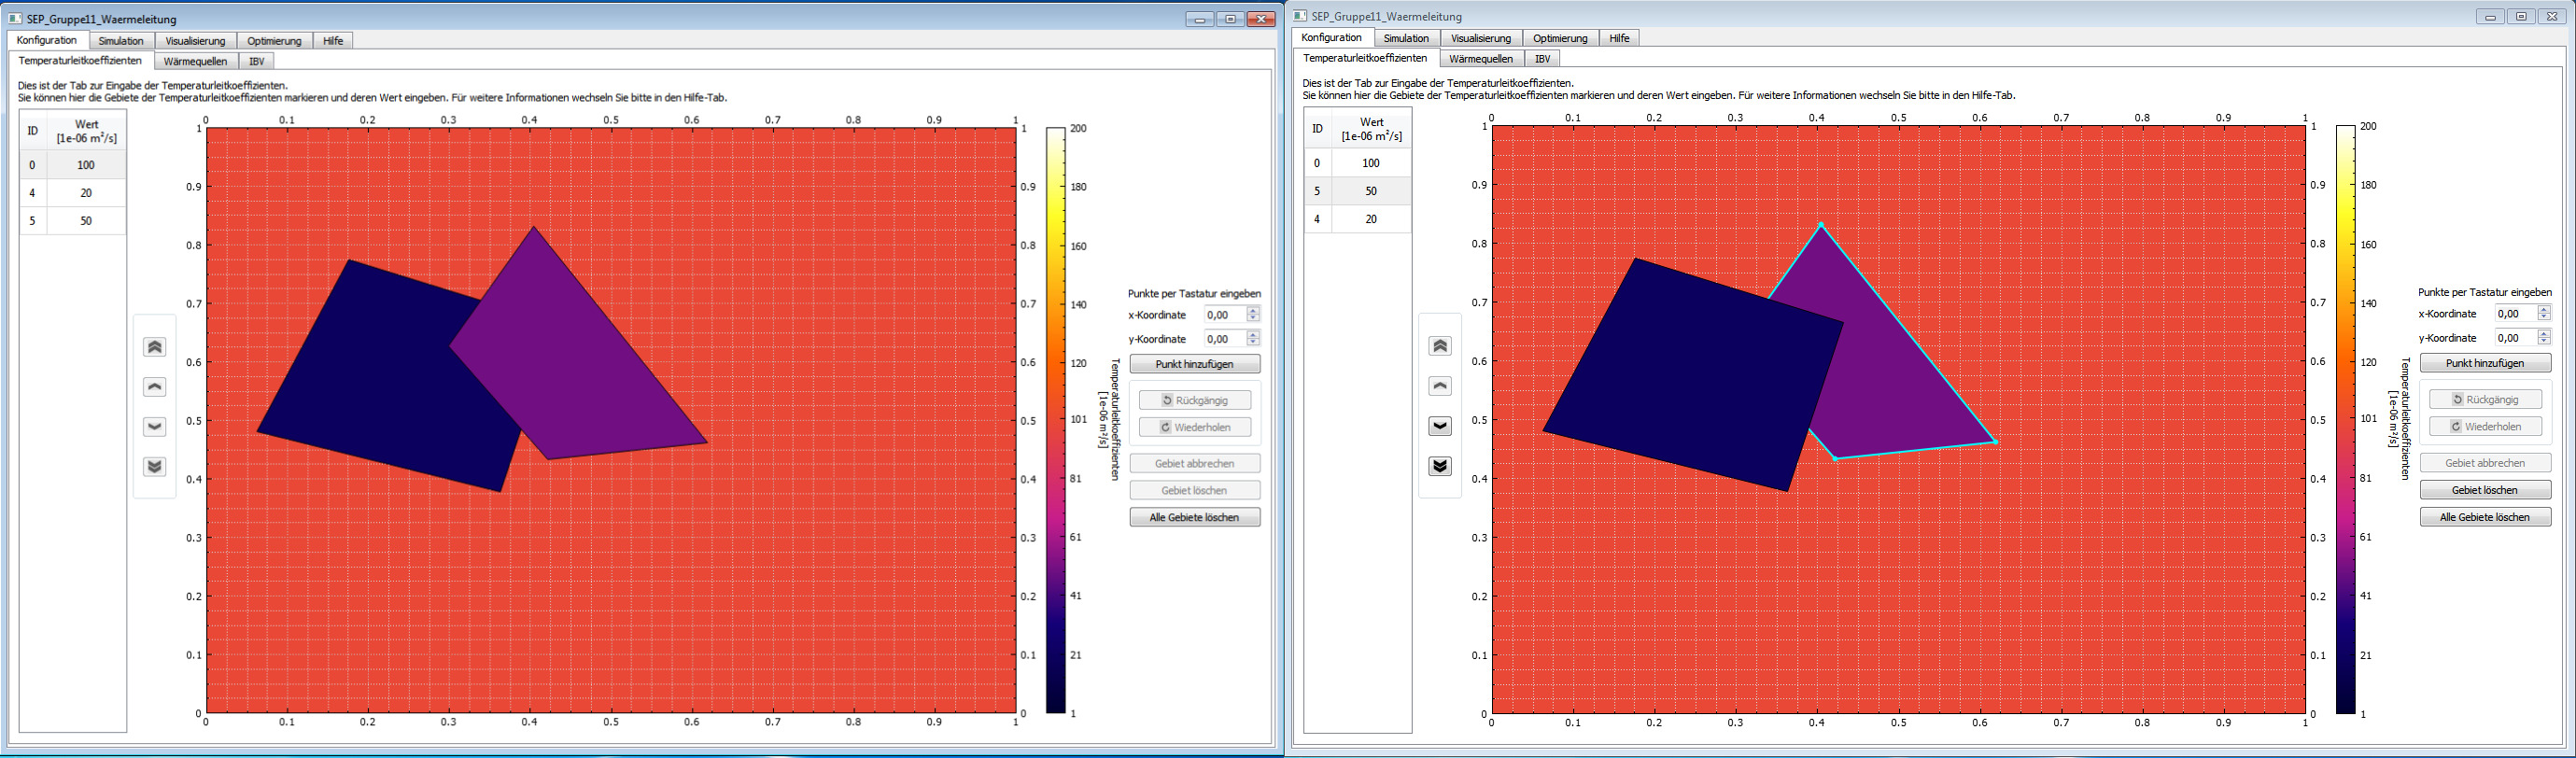
\includegraphics[scale=.25]{Bilder/ReihenfolgeAendern.png}\\
\caption{Reihenfolge ändern}
\label{ReihenfolgeAendern}
\end{figure}

\newpage
\noindent
Wert eines Gebietes ändern: Um den Temperaturleitkoeffizienten bzw den Wert der Wärmequelle eines Gebietes zu ändern, klicken Sie mit einem Doppelklick auf den Wert in der Tabelle in der Spalte 'Werte'. Anschließend wird das ausgewählte Gebiet auf der Platte markiert und Sie können den neuen Wert eingeben.
\begin{figure}[H]
\centering
%\hspace{-1.75cm}
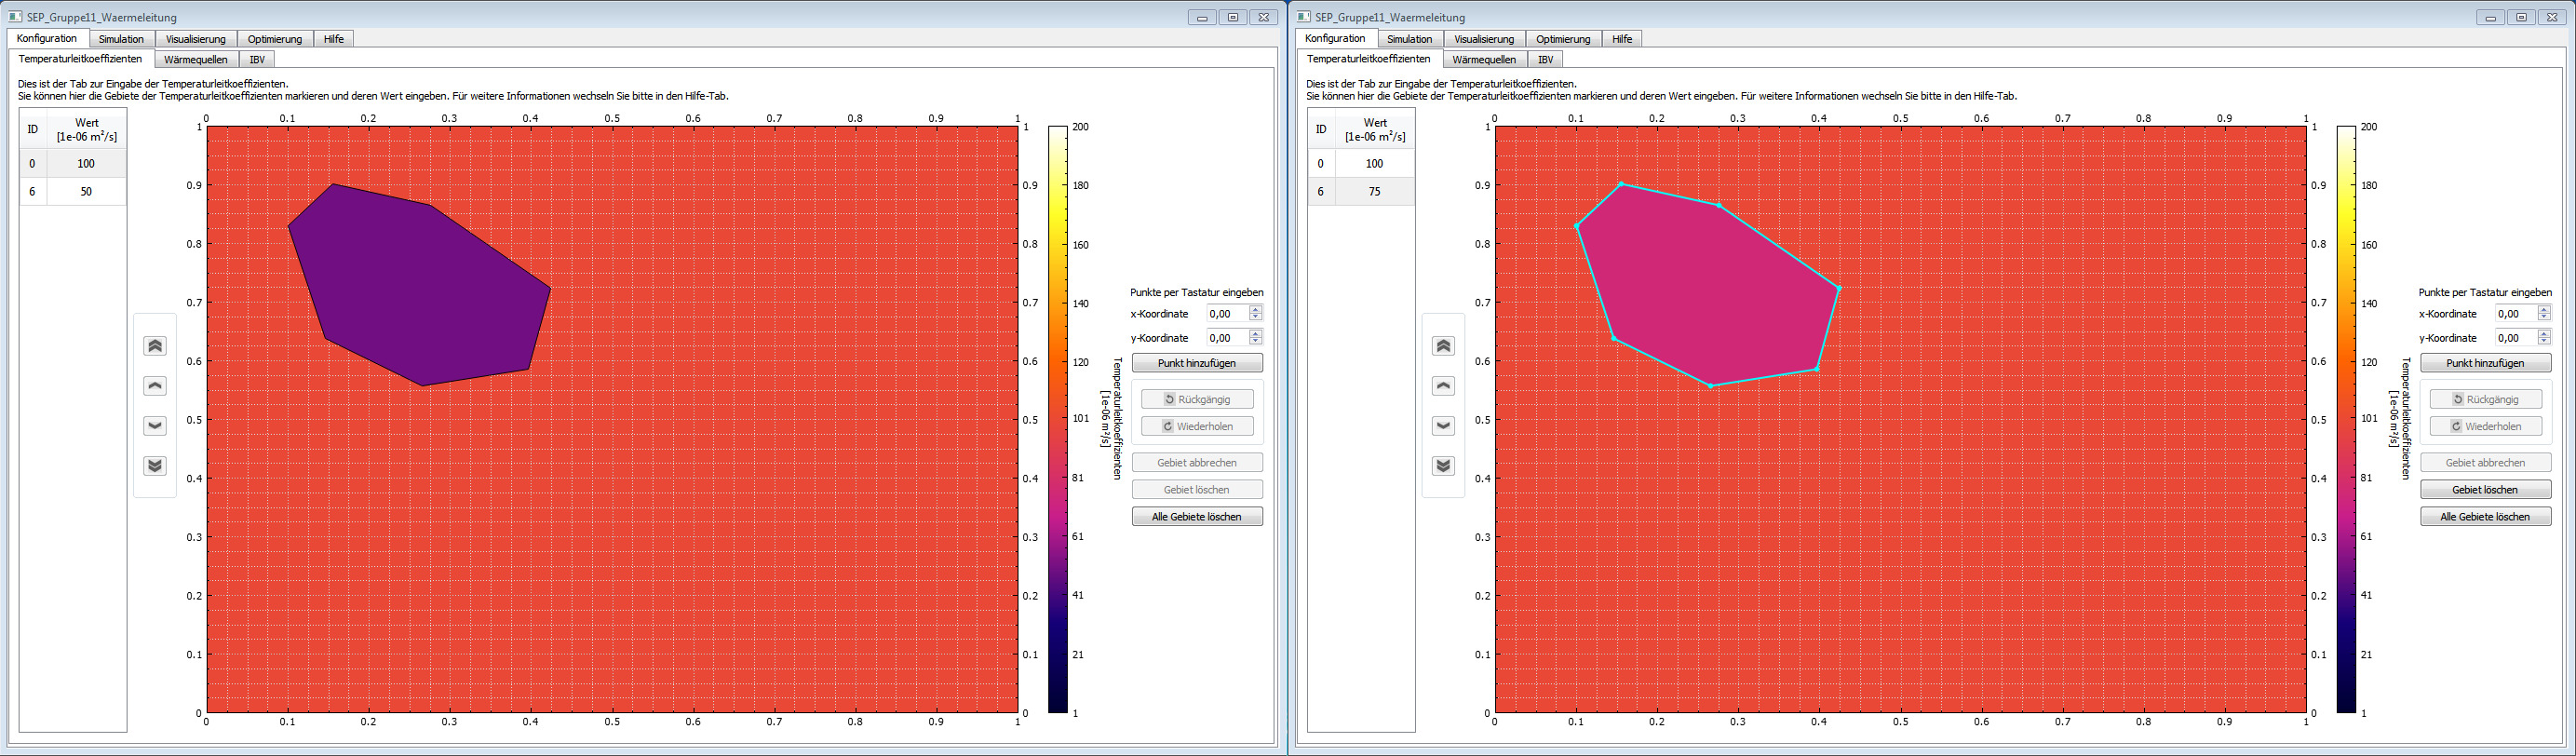
\includegraphics[scale=.25]{Bilder/WertAendern.png}\\
\caption{Wert eines Gebiets ändern}
\label{WertAendern}
\end{figure}

\noindent
Der dritte Tab ist zur Einstellung der Anfangs- und Randwerte.\\
Der IBV-Tab bietet Ihnen folgende Funktionalitäten:\\
Um die Anfangswerte und Randwerte zu ändern, ändern Sie den gewünschten Wert in den Feldern 'Anfangswert eingeben', 'unteren Randwert eingeben', 'linken Randwert eingeben', 'rechten Randwert eingeben' oder 'oberen Randwert eingeben'.
\begin{figure}[H]
\centering
%\hspace{-1.75cm}
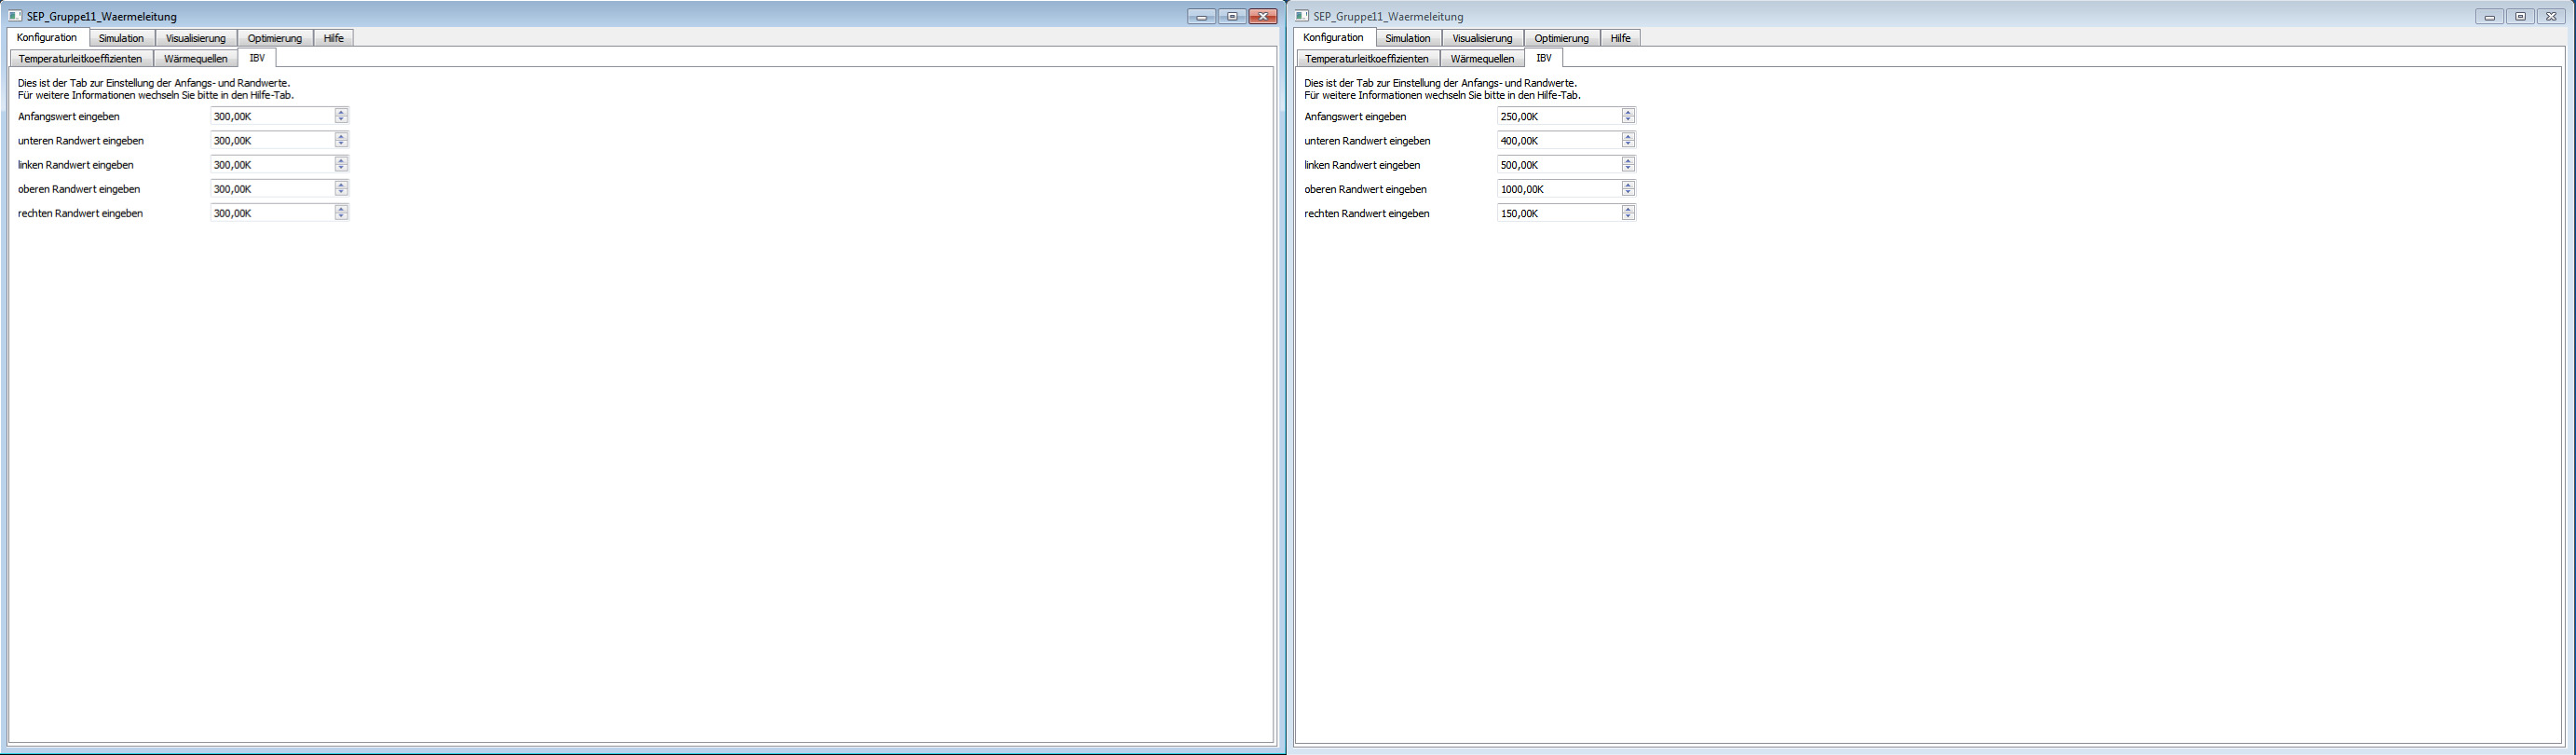
\includegraphics[scale=.25]{Bilder/IBVWerteAendern.png}\\
\caption{Anfangs- und Randwerte ändern}
\label{IBVWerteAendern}
\end{figure}

\newpage
\noindent
Der Simulations-Tab bietet Ihnen folgende Funktionalitäten:\\
\begin{enumerate}
\item Zeitdiskretisierung ändern:
In der Box 'Zeitdiskretisierung' können Sie die Integrationsmethode, die Zeitschritte M und den Endzeitpunkt T ändern.
\item Linearen Gleichungssystemlöser einstellen:
In der Box 'LGS Löser' können Sie den Löser, die relative Genauigkeit und die maximale Iterationszahl ändern.
\item Ortsdiskretisierung einstellen:
In der Box 'Ortsdiskretisierung' können Sie die Stützstellen N eingeben und die Simuation starten, indem Sie auf den Knopf 'Simulieren' drücken. Außerdem können Sie eine gestartete Simulation abbrechen, hier wird das Ergebnis der vorherigen Simulation ungültig.
\item Simulationseinstellungen:
In der Box 'Simulationseinstellungen' können Sie durch Klick auf den Knopf 'Speichern' alle gesetzten Einstellungen speichern. Ebenso können Sie zuvor gesetzte Einstellungen Laden, indem Sie auf den Knopf 'Laden' klicken. Indem Sie auf den Knopf 'Zurücksetzten' klicken, werden alle zuvor gemachten Einstellungen auf den Anfangszustand zurückgesetzt.
\end{enumerate}
\begin{figure}[H]
\centering
%\hspace{-1.75cm}
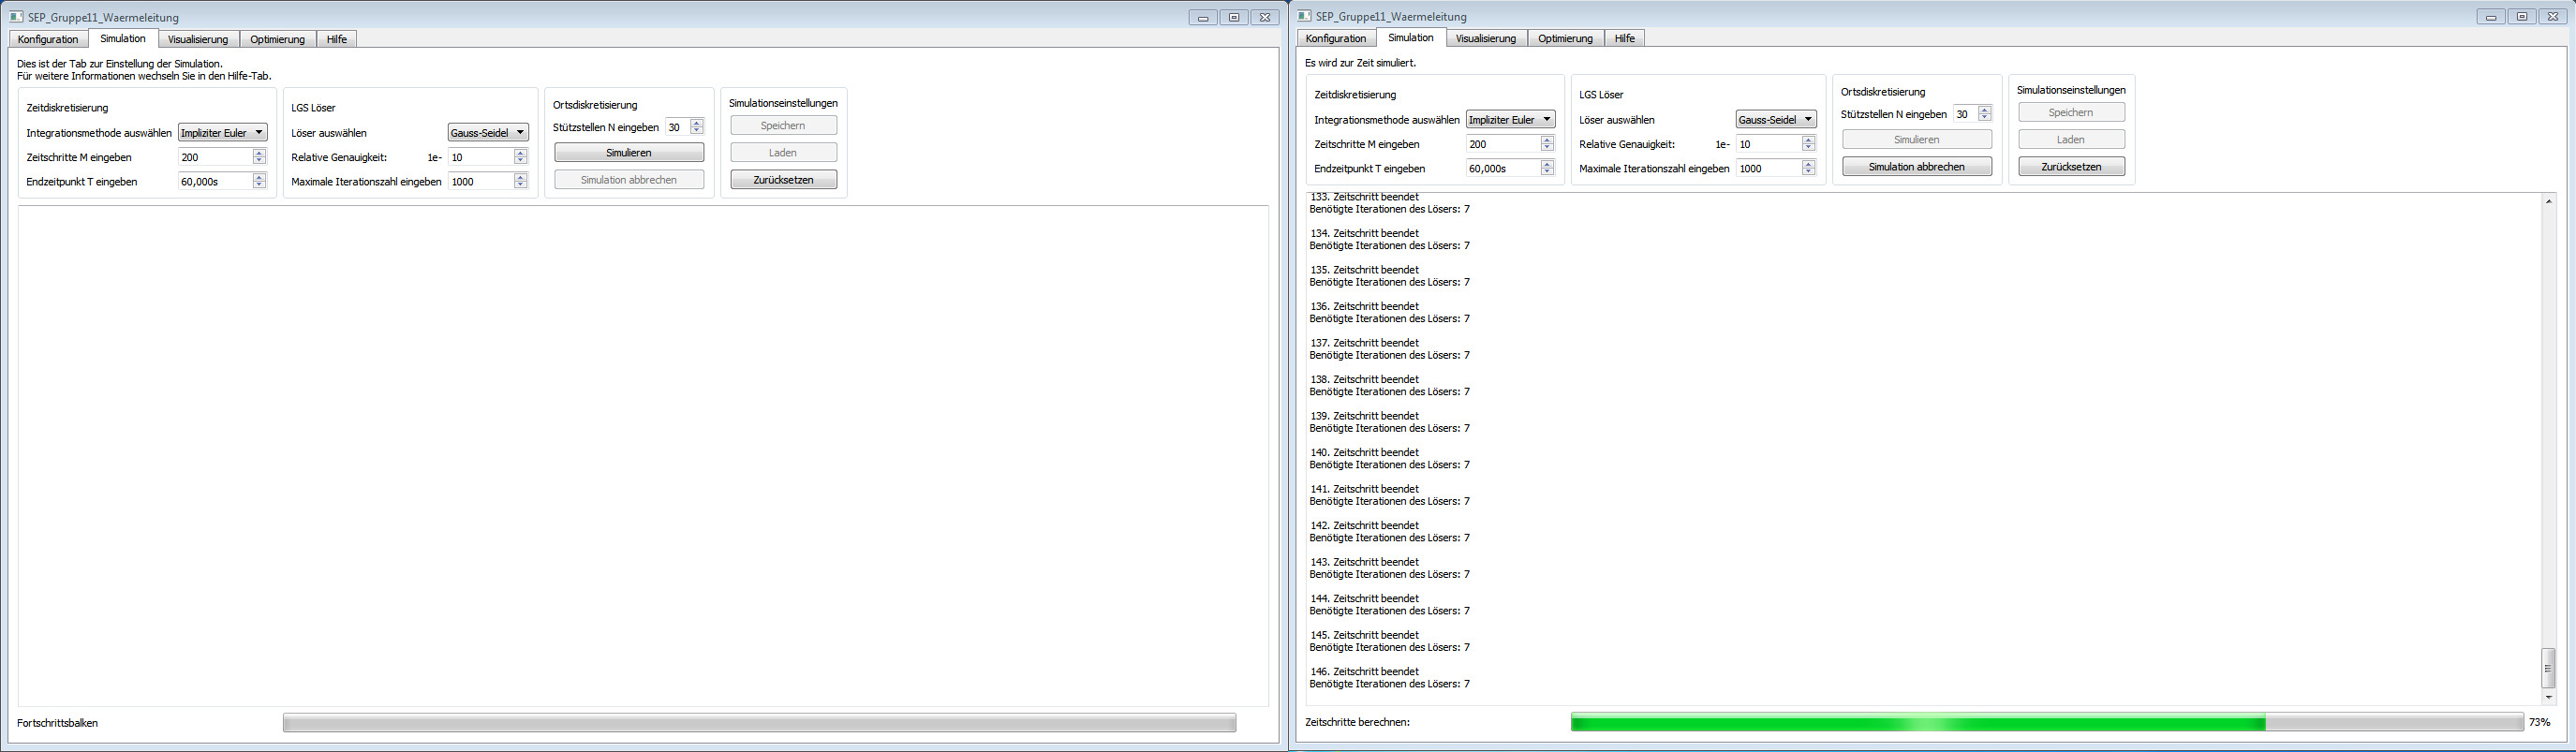
\includegraphics[scale=.25]{Bilder/SimulationStarten.png}\\
\caption{Start einer beliebigen Simulation}
\label{SimulationStarten}
\end{figure}


\newpage
\noindent
Der Visualisierungs-Tab bietet Ihnen folgende Funktionalitäten:\\
Nachdem eine Simulation erfolgreich angeschlossen worden ist, können Sie sich die Visualisierung der Temperaturverteilung als Video oder als Einzelbild anschauen.
\begin{enumerate}
\item Video starten: Um das Video zu starten, drücken Sie auf den Knopf 'Play'.
\item Bild anzeigen: Um ein Einzelbild anzeigen zu lassen, bewegen Sie den Schieberegler unter der Platte an die gwünschte Position.
\item Video versetzt anfangen lassen: Bewegen Sie den Schieberegler an die Positon von der Sie das Video starten möchten und klicken Sie anschließend auf den Knopf 'Play'.
\end{enumerate}
\begin{figure}[H]
\centering
%\hspace{-1.75cm}
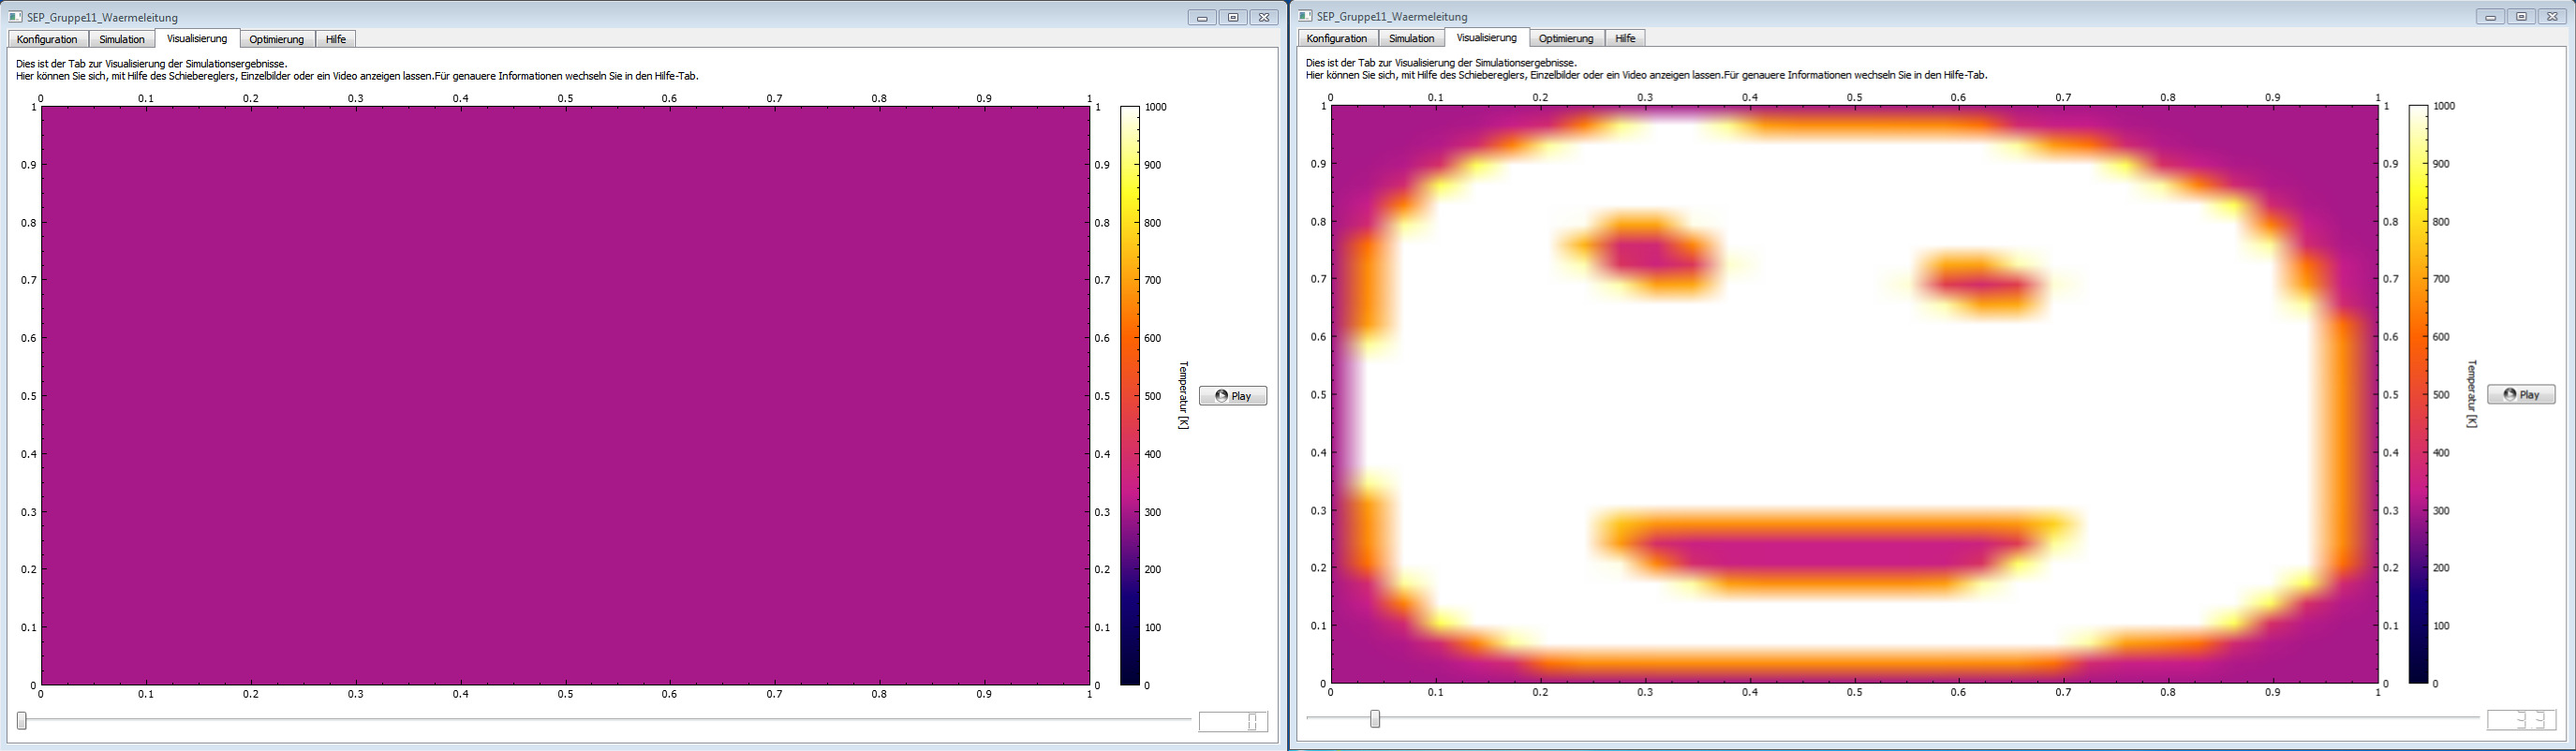
\includegraphics[scale=.25]{Bilder/Visualisieren.png}\\
\caption{Visualisierung eines beliebigen Zustands}
\label{Visualisieren}
\end{figure}


\newpage
\noindent
Der Optimierungs-Tab besteht aus zwei weiteren Tabs:\\

Der Konfigurations-Tab bietet Ihnen folgende Funktionalitäten:\\
\begin{enumerate}
\item Laden von Messungen/Beobachtungen: Indem Sie auf den Knopf 'Laden' klicken, können Sie Messungen/Beobachtungen einlesen lassen.
\item Vorhandene Wärmequellen nutzen: Indem Sie die Checkbox 'Nutze bereits vorhandene Wärmequellen zur Simulation' aktivieren, werden die eingegebenen Wärmequellen aus dem Tab Wärmequellen für die Simulation übernommen.
\item Anfangs Temperaturleitkoeffizienten ändern: Um die Anfangs Temperaturleitkoeffizienten zu ändern, aktivieren Sie die Checkbox 'Überschreibe bereits vorhandene Temperaturleitkoeffizienten zur Simulation' und ändern Sie anschließend den Wert im entsprechenden Feld.
\item Simuationseinstellungen ändern: Um die Simuationseinstellungen zu ändern wechslen Sie in den Simulations-Tab und ändern Sie dort die gewünschten Werte.
\item Optimierung starten: Indem Sie auf den Knopf 'Optimierung starten' klicken, wird die Optimierung gestartet und anhand eines Fortschrittsbalken wird der Fortschritt angezeigt.
\end{enumerate}
\begin{figure}[H]
\centering
%\hspace{-1.75cm}
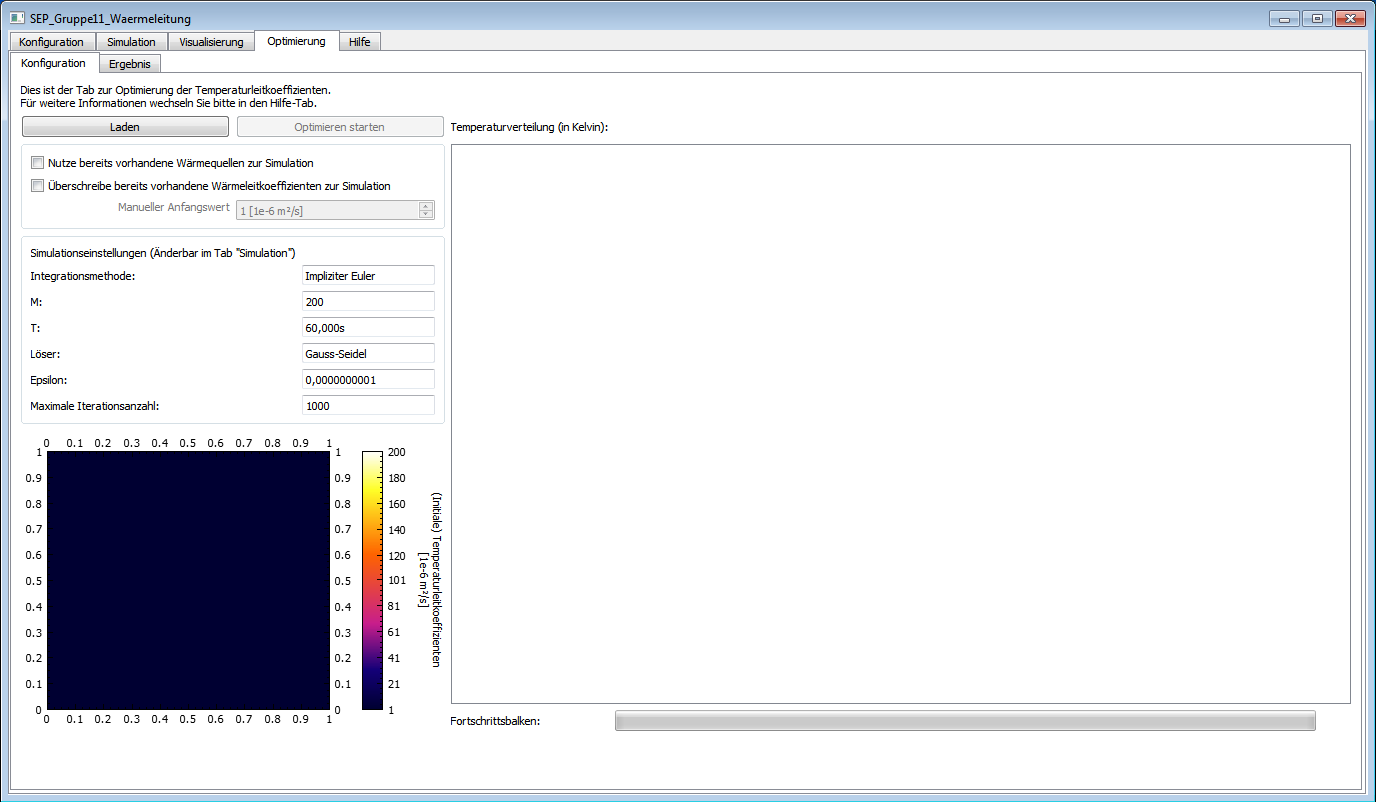
\includegraphics[scale=.25]{Bilder/OptimierungStarten.png}\\
\caption{Optimierung starten}
\label{OptimierungStarten}
\end{figure}

Der Ergebnis-Tab zeigt die gefitteten Temperaturleitkoeffizienten in Form einer Tabelle an.
\begin{figure}[H]
\centering
%\hspace{-1.75cm}
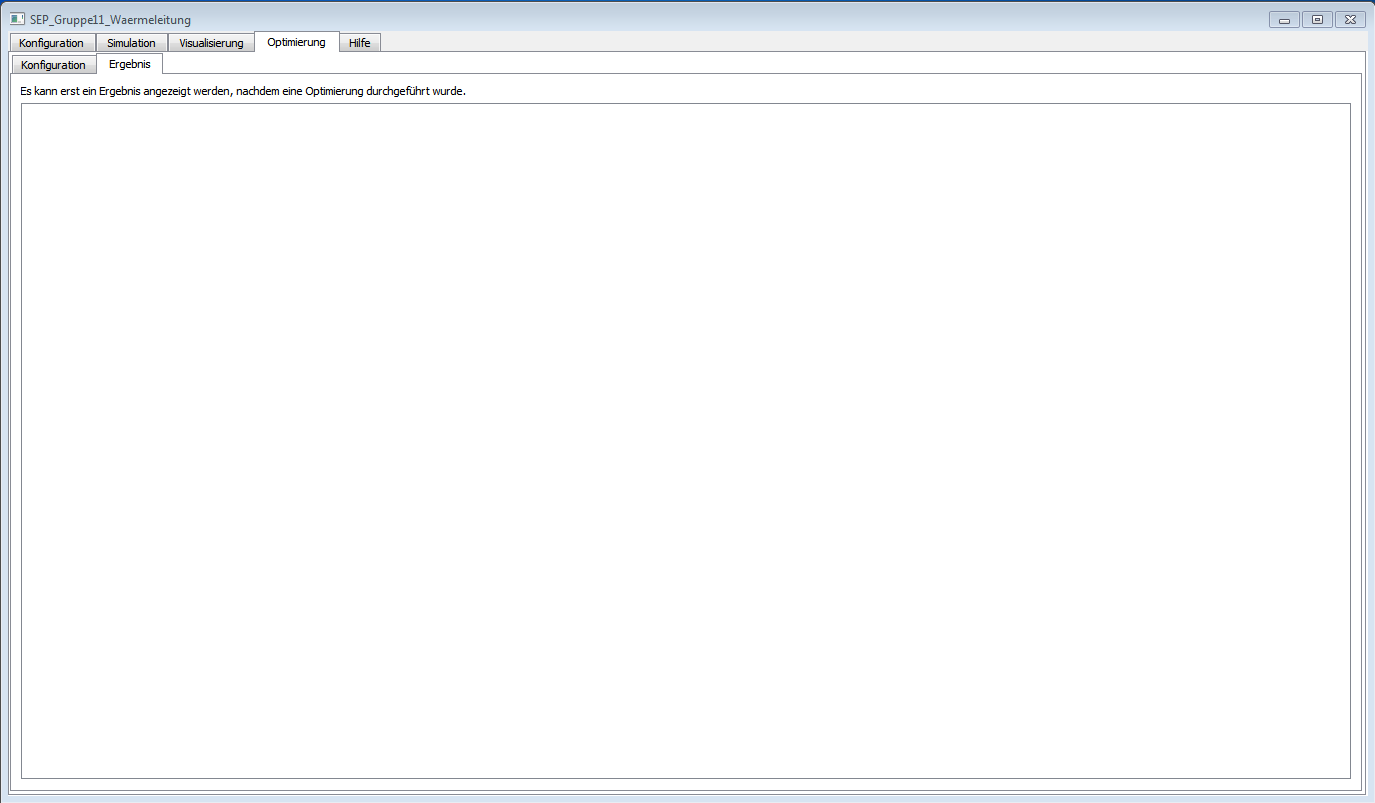
\includegraphics[scale=.25]{Bilder/ErgebnisAnzeigen.png}\\
\caption{gefitteten Temperaturleitkoeffizienten}
\label{ErgebnisAnzeigen}
\end{figure}



\newpage
\section{Fehlersituationen}

Während der Benutzer ein Gebiet eingibt, darf er den Tab nicht wechseln.
\begin{figure}[H]
\centering
%\hspace{-1.75cm}
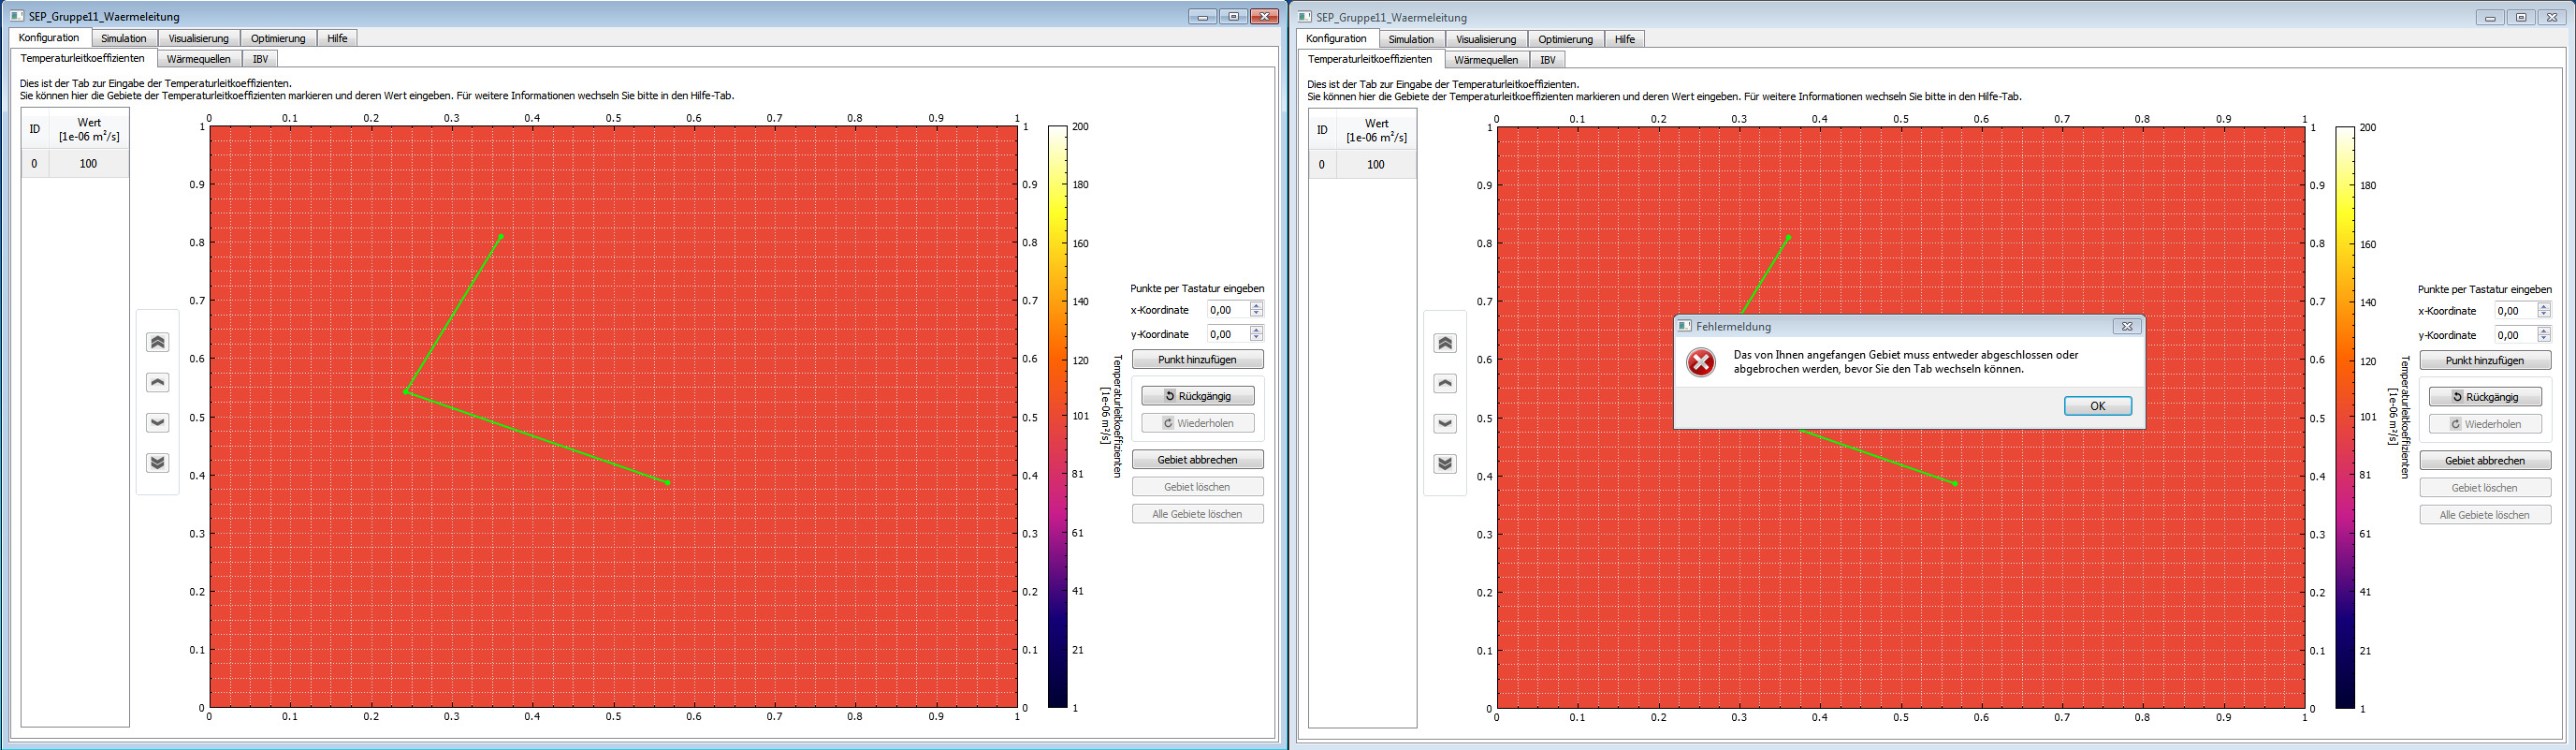
\includegraphics[scale=.25]{Bilder/FehlerTabWechseln.png}\\
\caption{Fehler Tab Wechseln}
\label{FehlerTabWechseln}
\end{figure}

\noindent
Ein korrektes Gebiet muss einfach wegzusammenhängend sein, d.h. Kanten dürfen sich nicht schneiden.
\begin{figure}[H]
\centering
%\hspace{-1.75cm}
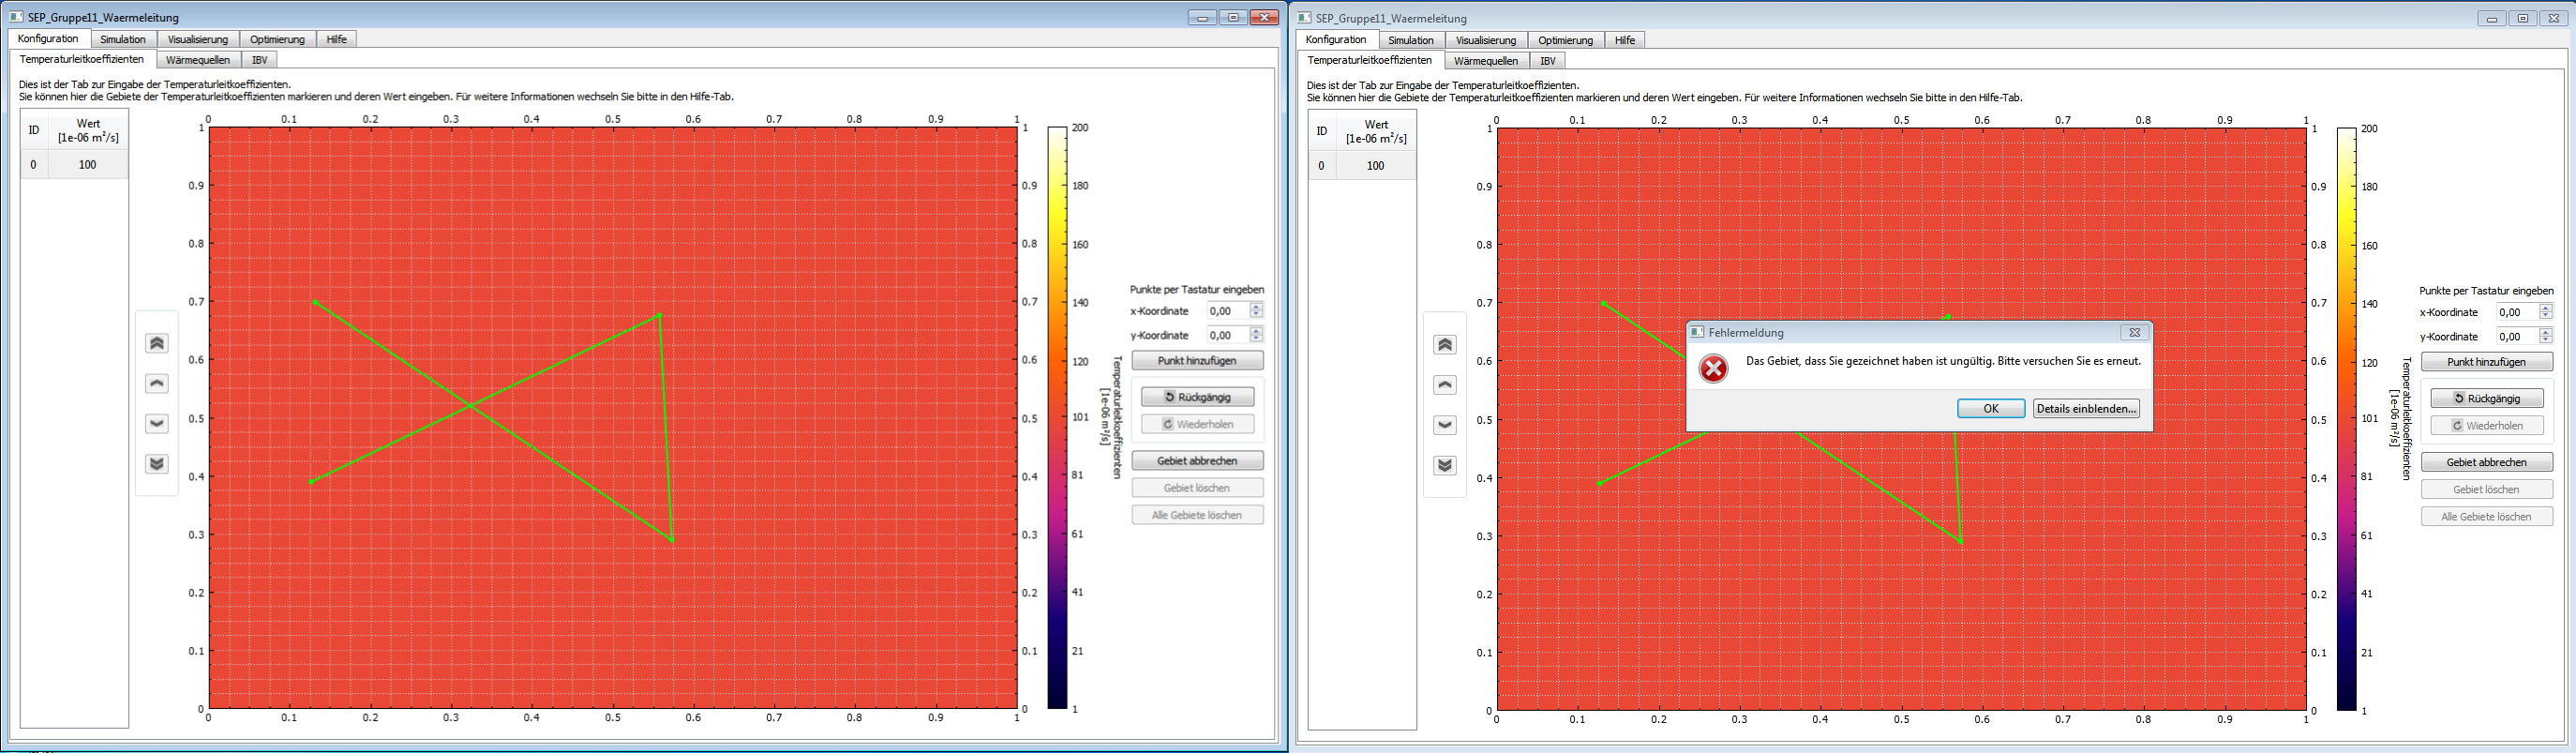
\includegraphics[scale=.25]{Bilder/FehlerGebietEingeben.png}\\
\caption{Fehler Gebiet eingeben}
\label{FehlerGebietEingeben}
\end{figure}